\documentclass[a4paper,11pt]{article}
\usepackage[a4paper, total={6in, 8in}]{geometry}
\usepackage[T1]{fontenc}
\usepackage[utf8]{inputenc}
\usepackage[english,serbian]{babel}
\usepackage{graphicx}
\usepackage{subfig}
\usepackage{fancyhdr}

\renewcommand{\figurename}{Slika}
\graphicspath{ {./img/} }

\title{Smerač}
\author{Aleksa Siriški}
\date{Novembar 2022}

\begin{document}

\pagestyle{empty}
\begin{center}
    \begin{figure}
        \centering
        
\includegraphics[height=3cm,width=3cm]{pmf}
    \end{figure}

    \textbf{
    UNIVERZITET U NOVOM SADU
    \\
    PRIRODNO-MATEMATIČKI
    \\
    FAKULTET
    \\
    DEPARTMAN ZA MATEMATIKU
    \\
    I INFORMATIKU
    }

\end{center}
\vfill
\begin{center}
	\begin{huge}
		\textbf{Smerač}
		\bigskip 
	\end{huge}
	\\
	\begin{large}
        \textbf{- seminarski rad iz predmeta Skript jezici -}
	\end{large}
\end{center}
\vfill
\begin{center}
    Aleksa Siriški, 159/22
    \\
    Novi Sad, 2022.
\end{center}
\newpage

\pagestyle{plain}
\renewcommand{\contentsname}{Sadržaj}
\addcontentsline{toc}{section}{Sadržaj}
\tableofcontents
\newpage

\pagestyle{fancy}
\lhead{Smerač}
\rhead{Aleksa Siriški}
\cfoot{\thepage}

\section{Uvod}
\subsection{Discord}
Discord\cite{discord}, kao jedna od najpopularnijih društvenih mreža za programere i entuzijaste računarskih tehnologija, je logičan izbor za razmenu informacija i raspoređivanje časova IT i RN smerova Univerziteta u Novom Sadu. Uprkos jednostavnosti Discord-ovog grafičkog interfejsa nije lako omogućiti studentima da sami sebi određuju smer a direktna integracija sa Google kalendarom je apsolutno neizvodljiva. Na sreću, Discord tim je osposobio trećim licima da kreiraju 'Bot' naloge i uz pomoć njihovog REST API će nastati Smerač - Discord Bot stvoren da omogući studentima izbor sopstvenog smera kao i integraciju Google kalendara.
\subsection{Python}
Smerač je Python\cite{python} skripta napisana u svega 300 linija koda. Računajući da korisnicima nije bitno da li će im smer biti dodeljen za 1ms ili 1s Python je bio prikladan izbor. Najpre zbog mnogobrojnih ugrađenih biblioteka i modula, kao što su interactions-py\cite{interactions-py} i asyncio\cite{asyncio}, ali i zbog jednostavne sintakse koja je omogućila eksponencijalan razvoj ovog programa.
\subsection{Ideja}
Discord bot koji mora biti dovoljno jednostavan ali isto tako i univerzalno programiran da se može lako primeniti na više različitih okruženja (Discord servera). Takva prilagodljivost se postiže pametnim planiranjem toka rada programa i korišćenjem promenljivih okruženja (eng. \textit{environment variables}). Takođe je jako bitna licenca koja će se koristiti, da ne bi došlo do krađe autorskih prava i zloupotrebe softvera. Tačno iz tih razloga odabrana licenca za Smerač će biti GNU General Public License\cite{gpl}.
\subsection{Asinhronizacija}
Kako bi program mogao da istovremeno čita poruke od različitih korisnika potrebno je kreiranje dodatnih niti. Pomoću biblioteke asyncio Smerač će imati mogućnost paralelnog parsiranja kalendara i dodeljivanja smera svakom studentu koji to zatraži. Pored bržeg izvođenja programa asinhrone funkcije služe da oduzmu čekanje odgovora od servera, tj. ako zahtev prvog korisnika traje duže da se obradi drugi korisnici ne moraju da čekaju nego se i njihovi zahtevi obrađuju u istom trenutku.
\subsection{Smerovi}
Najbitnija i najjednostavnija funkcionalnost Smerača će biti dodeljivanje smera studentima. Program će izvršavati korisničke komande oblika:
\begin{verbatim}
/smer <naziv_smera>
\end{verbatim}
gde je <naziv\_smera> IT/RN/PM i dodeljivati odgovarajući smer tom studentu.
\newpage

\subsection{Kalendar}
Učitavanje podataka iz Google-ovog kalendara će biti omogućeno zahvaljujući postojanju JSON objekta proizvoljnog kalendara koji je nalik ugrađenim rečnicima u Python-u. Uprkos lakom učitavanju potrebno je kompleksnije parsiranje kalendara, naime jedno string polje 'summary' sačinjava naziv predmeta, profesor, tip časa kao i mesto odvijanja. Smerač će to parsiranje izvesti na što efikasniji način sa minimalnim brojem petlji i korišćenjem ugrađenih i optimalnih funkcija za rad sa stringovima.
\\\\
Nakon uspešno parsiranih podataka potrebno je generisati raspored prilagođen za čitanje na računarima i telefonima. Smerač će spojiti istoimene predmete ali će zapisati odvojene termine časova u zavisnoti od profesora koji ga drži kao i mesta odvijanja nastave. Primer ispisa se može videti na Slici a. Pored tekstualnog ispisa Smerač će od istih podataka generisati stubičasti grafik koji omogućava lakši prikaz broja časova na dnevnom nivou, primer toga se nalazi na Slici b.
\begin{figure}[h]
    \centering
    \subfloat[Parsiran i uređen raspored časova za sredu, IT smer]{{
\includegraphics[height=8cm,width=5cm]{sreda} }}
    \hspace{1cm}
    \subfloat[Grafik sa dnevnim prikazom časova, IT smer]{{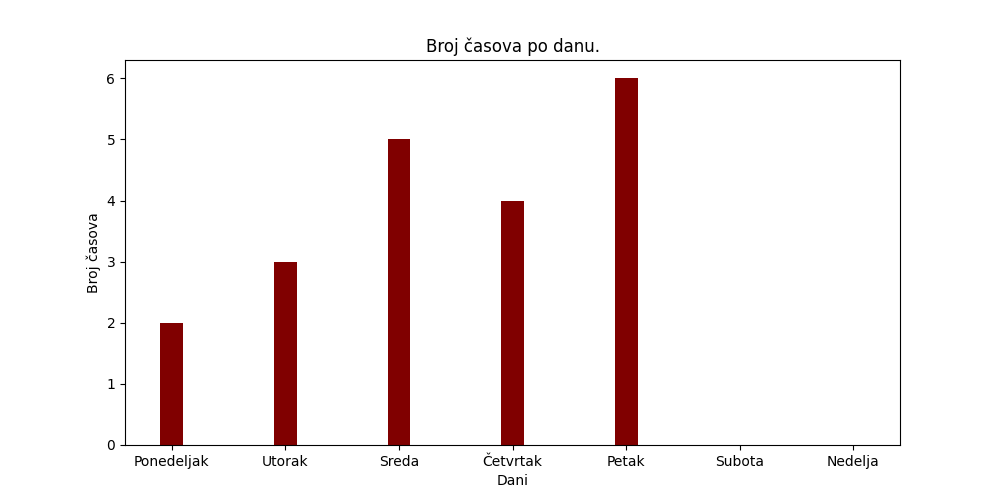
\includegraphics[height=5cm,width=7cm]{it} }}
\end{figure}
\newpage

\section{Opis programa}
\subsection{Nagli prekid usled greške}
Ovaj deo koda služi da prekine tok programa u potpunosti, najčešće se koristi prilikom učitavanja promenjlivih okruženja tj. u slučaju da nisu postavljene.
\begin{verbatim}
    def fail(msg):
        print(msg)
        exit(1)
\end{verbatim}
\subsection{Promenljive okruženja}
Da bi Smerač mogao učitati potrebne postavke, koristi se biblioteka \textit{OS}. U sledećem kodu se takođe može videti upotreba naglog prekida kao i korišćenje nekih podrazumevanih vrednosti.
\begin{verbatim}
    def setup_config():
        config = dict()

        ...

        COMMAND = os.getenv("COMMAND")
        if COMMAND == None:
            COMMAND = "smer"
        config["command"] = COMMAND

        ...

        DISCORD_TOKEN = os.getenv("DISCORD_TOKEN")
        if DISCORD_TOKEN == None:
            fail("DISCORD_TOKEN env isn't set")
        config["discord_token"] = DISCORD_TOKEN

        NUMBER_OF_ROLES = int(os.getenv("NUMBER_OF_ROLES"))
        if NUMBER_OF_ROLES == None:
            fail("NUMBER_OF_ROLES env isn't set")

        ...

        return config
\end{verbatim}
\newpage
\subsection{Logging}
Jedna od krucijalnih funkcionalnosti svakog programa je mogućnost zapisivanja šta se dešava prilikom izvršavanja. To je najpotrebnija alatka prilikom debagovanja koda, bilo to starog ili novog koda neke naknadno dodate funcionalnosti.
\begin{verbatim}
def setup_config():
    
    ...

    LOG_FILE = os.getenv("LOG_FILE")
    if LOG_FILE == None:
        LOG_FILE = "/config/logs/%s.log"
                   %(datetime.today().strftime("%Y-%m-%d-%H-%M-%S"))
    config["log_file"] = LOG_FILE
    
    ...
\end{verbatim}
\begin{verbatim}
def setup_logger(config):
    if os.getenv("DEBUG") == None:
        logging_level = logging.INFO
    else:
        logging_level = logging.DEBUG

    logging.basicConfig(
        filename=config["log_file"],
        level=logging_level,
        format=
        "%(asctime)s - %(name)s[%(process)s] - %(levelname)s - %(message)s",
    )
\end{verbatim}
\subsection{Globalne promenljive}
Globalne promenljive su potrebne isključivo kada sve funkcije, iz celog programa, zahtevaju čitanje i pisanje zajedničkih podataka. Odličan primer ovoga bi bila konfiguracija sa svim postavkama potrebnim za rad programa. Pored toga, koristi se i promenljiva \textit{log} i \textit{bot} koja služi da se interaguje sa interactions-py API.
\begin{verbatim}
    log = logging.getLogger("smerac")
    config = setup_config()
    bot = interactions.Client(token=config["discord_token"])
\end{verbatim}
\newpage
\subsection{Slash komande}
\textit{Slash komande} se zapisuju u obliku:
\begin{verbatim}
    /<naziv_komande> [opcija_1] [opcija_2] ...
\end{verbatim}
Takve komande su standardizovan način pozivanja funkcija proizvoljnog Discord bota.
\subsubsection{Kreiranje slash komande}
Pomoću biblioteke interactions-py moguće je kreirati slash komandu sa nazivom \textit{smer} i obaveznom opcijom \textit{traženi\_smer}, Slika a:
\begin{verbatim}
    @bot.command(
        name="smer",
        description="Choose your role!",
        options = [
            interactions.Option(
                name="wanted_role",
                description="The role you want.",
                type=interactions.OptionType.STRING,
                required=True,
            ),
        ],
    )
\end{verbatim}
\begin{figure}[h]
    \centering
    \subfloat[Slash komanda na Discordu]{{
\includegraphics[height=2.5cm,width=6cm]{slashcommand}}}
\end{figure}
\newpage
\subsubsection{Dodeljivanje funkcionalnosti slash komandi}
Da bi kreirana slash komanda izvršavala neki kod potrebno je odmah ispod njene kreacije deklarisati asinhrohu funkciju koja će izvršavati željeni kod.
\begin{verbatim}
async def choose_role(ctx: interactions.CommandContext, wanted_role: str):
    author = ctx.author

    log.debug(f"Started choosing role for {author.nick}")

    guild = await ctx.get_guild()
    discord_roles = await guild.get_all_roles()

    for author_role_id in author.roles:
        author_role = await guild.get_role(author_role_id)
        for role in config["roles"]:
            if role.upper() == author_role.name.upper():
                await author.remove_role(author_role_id)
                log.debug(f"Removed {author.nick} from {role}")
            else:
                log.debug(f"Role {role} isn't {author_role.name}")
    
    if wanted_role != "none":
        for role in config["roles"]:
            if wanted_role.upper() == role.upper():
                for discord_role in discord_roles:
                    if wanted_role.upper() == discord_role.name.upper():
                        await author.add_role(discord_role.id)
                        break
                break
        log.info(f"Added {author.nick} to {wanted_role}.")
        await ctx.send(f"Succesfully added {author.nick} to 
                                                    {wanted_role.upper()}!",
                                                             ephemeral=True)
    else:
        log.info(f"Removed {author.nick} from all roles.")
        await ctx.send(f"Succesfully removed {author.nick} from all roles!",
                                                             ephemeral=True)
\end{verbatim}
\newpage
test
\newpage
\section{Zaključak}
test
\newpage

\pagestyle{plain}
\renewcommand\refname{Literatura}
\addcontentsline{toc}{section}{Literatura}
\bibliography{references}
\bibliographystyle{ieeetr}

\end{document}